\documentclass{sciposter}
\usepackage{lipsum}
\usepackage{epsfig}
\usepackage{amsmath}
\usepackage{amssymb}
\usepackage{multicol}
\usepackage{graphicx,url}
\usepackage[spanish]{babel}   
\usepackage[utf8]{inputenc}
%\usepackage{fancybullets}
\newtheorem{Def}{Definition}


\title{Reconocimiento de actividades humanas con un enfoque colaborativo}
%Título do projeto

\author{Alberto Gimenez, Santiago A. Yegros Z, Joaquín Lima}
%nome dos autores

\institute 
{Facultad Politécnica - Universidad Nacional de Asunción \\
  San Lorenzo, Paraguay}
%Nome e endereço da Instituição

\email{{albergimenez@gmail.com, santiago.yegros@gmail.com, joaquin.lima@pol.una.py}}
% Onde você coloca os emails dos integrantes


%\date is unused by the current \maketitle

\rightlogo[1]{logo}
\leftlogo[1]{logo.jpg}
% Exibe os logos (direita e esquerda) 
% Procure usar arquivos png ou jpg, e de preferencia mantenha na mesma pasta do .tex
%%%%%%%%%%%%%%%%%%%%%%%%%%%%%%%%%%%%%%%%%%%%%%%%%%%%%%%%%%%%%%%%%%%%%%%%%%%%%%%%
%%% Begin of Document



\begin{document}
%define conference poster is presented at (appears as footer)

\conference{Diciembre 2017}

%\LEFTSIDEfootlogo  
% Uncomment to put footer logo on left side, and 
% conference name on right side of footer

% Some examples of caption control (remove % to check result)

%\renewcommand{\algorithmname}{Algoritme} % for Dutch

%\renewcommand{\mastercapstartstyle}[1]{\textit{\textbf{#1}}}
%\renewcommand{\algcapstartstyle}[1]{\textsc{\textbf{#1}}}
%\renewcommand{\algcapbodystyle}{\bfseries}
%\renewcommand{\thealgorithm}{\Roman{algorithm}}

\maketitle

%%% Begin of Multicols-Enviroment
\begin{multicols}{3}

%%% Abstract
\begin{abstract}
Human Activity Recognition (HAR) es un tema de investigación ampliamente cubierto en la última década por su relevancia en áreas donde el contexto de los usuarios es importante para construir aplicaciones interactivas. Las aplicaciones móviles para teléfonos inteligentes tienen la capacidad de capturar datos del entorno por medio de sensores y en conjunción con algoritmos que aprovechan la información sensible al contexto, se convierten en una poderosa plataforma de desarrollo. En este trabajo, proponemos un sistema HAR denominado HARDroid que está específicamente diseñado para detectar actividades comunes de los usuarios. Además, los datos recopilados de los usuarios en pruebas de campo se tienen en cuenta para mejorar el clasificador de reconocimiento de actividad. HARDroid está disponible gratuitamente como una biblioteca que puede incluirse en las aplicaciones de Android. Finalmente, se presenta una evaluación que compara el clasificador inicial con un clasificador mejorado, logrando una exhaustividad del 91.34 \% y una precisión del 92.04 \%.
\end{abstract}

%%% Introduction
\section{Introducción}
A importância do assunto deve ser destacada resumidamente.

\PARstart{G}{ranulometries} are ordered sets of morphological openings or closings, each of
which removes image details below a certain size. These can be used for texture
analysis
through the use of \emph{pattern spectra}, which show how the number of 
foreground pixels in the image changes as a function of the size parameter 
\cite{maragos89:_patter}.
A drawback of the classical definition of pattern spectra is that spatial 
information is not included in a pattern spectrum as shown below.
 In this paper, \emph{spatial pattern spectra} are developed which retain information on the distribution of these details at different scales.
 

\newcommand{\imsize}{0.45\columnwidth}
\begin{figure}
\begin{center}
\begin{tabular}{c c}

\end{tabular}
\end{center}
\caption{ Parts (a) through (c) show three images consisting of squares of
different sizes;
(d) shows the pattern spectra, denoting the number of foreground pixels 
 removed by openings by reconstruction by $\lambda \times \lambda$ squares. No 
granulometry is capable of separating the patterns, because the only 
differences between the images lie in the distributions of the 
connected components. }\label{fig:blocks}
\end{figure}




\section{Metodología HAR}
Dar uma ideia compacta da metodologia ou forma de abordagem da pesquisa, bem como o projeto foi desenvolvido.\\

\begin{figure}
	\centering
	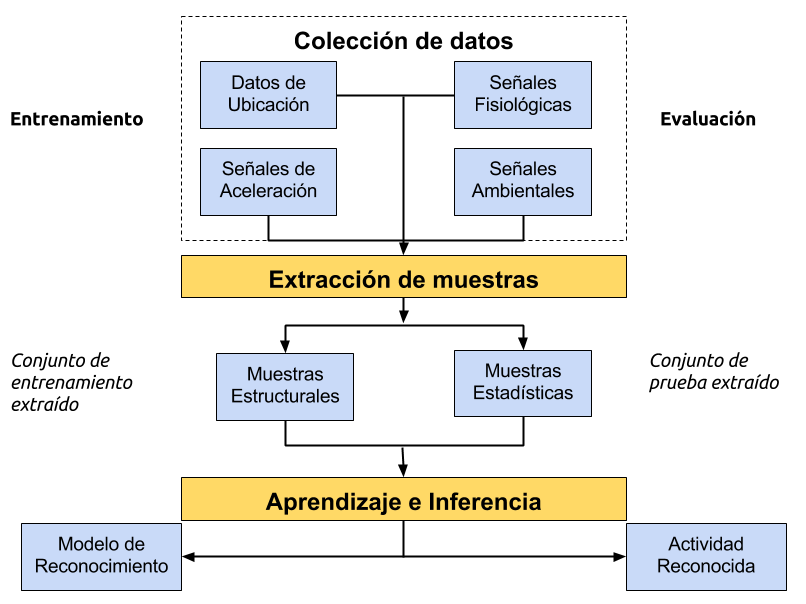
\includegraphics[width=0.7\linewidth]{../capitulo-2/graphics/harsystem}
	\caption{}
	\label{fig:harsystem}
\end{figure}


The opening transform \cite{Nacken:thesis} $\Omega_X$ of a binary image $X$ 
for a granulometry ${\alpha_r}$ is
\begin{equation}
  \Omega_X(x) = \max\{ r \in \Lambda \vert x \in \alpha_r(X) \}
\end{equation}

\begin{figure}
	\centering
	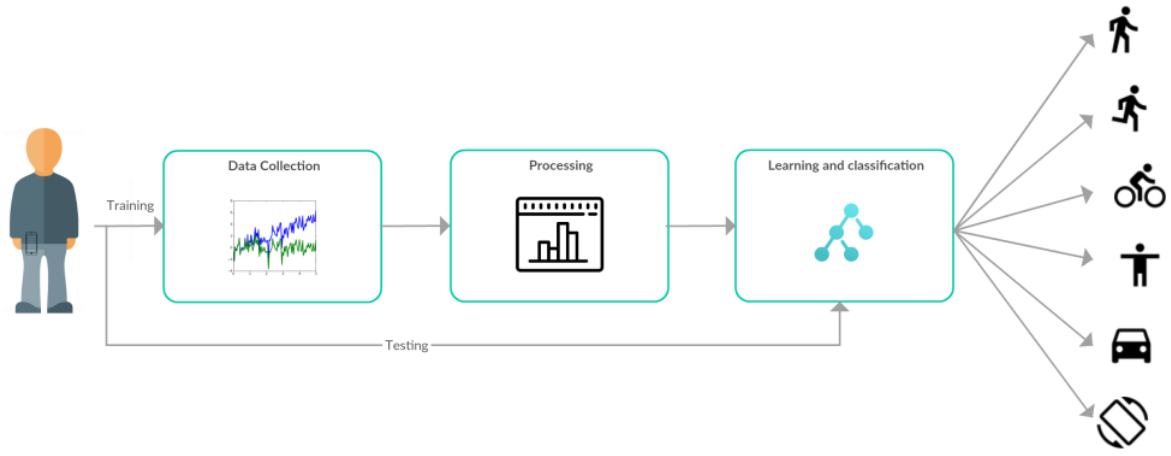
\includegraphics[width=0.7\linewidth]{../capitulo-2/graphics/harsystem2}
	\caption{}
	\label{fig:harsystem2}
\end{figure}


The pattern spectrum of a binary image $X$ using granulometry 
$\{\alpha_r\}$ is the histogram of $\Omega_X$ obtained with the same 
size distribution \cite{Nacken:thesis}, disregarding the bin for grey level 0.


\begin{figure}
\begin{center}
\end{center}
\caption{ \label{fig:opentransf} Opening transform with $\{\alpha_r\}$ as in 
 Fig. \ref{fig:blocks}: (left) original image; (right) opening transform
(contrast stretched for clarity). 
}
\end{figure}


\section{HARDroid}
Dar uma ideia compacta da metodologia ou forma de abordagem da pesquisa, bem como o projeto foi desenvolvido.
\\
Pattern spectra only retain the amount of detail present at  scale $r$.
This can be amended by computing some parameterization of the spatial 
distribution in an image $\alpha_r(X) \setminus \alpha_{r+}(X)$ as a function of $r$. 



An obvious parameterization of the spatial distribution is through 
the use of moments. Focusing on the case of 2-D binary images, the 
moment $m_{ij}$ of order $ij$ of an image $X$ is given by

  
These two are shown in Figures \ref{fig:tauspect} and \ref{fig:binspect}. Note that 
these definitions hold only where $(S_{m_{00},\alpha}(f))(r) \neq 0$. For all 
other values of $r$ they will be defined as zero. Further post-processing can
be done to compute central moments and moment invariant from pattern moment 
spectra \cite{Flusser:Suk:93,Hu:62}. 

\section{Resultados}

Verificar os principais resultados obtidos de acordo com os objetivos propostos.\\

Nacken \cite{Nacken:thesis} derived an algorithm for computation
of pattern spectra for granulometries based on openings by discs of increasing
radius for various metrics, using the opening transform. After the
opening transform has been computed, it is straightforward to compute the 
pattern spectrum:
\begin{itemize}
\item Set all elements of array {\tt S} to zero
\item For all $x \in X$ increment {\tt S}[$\Omega_X(x)$] by one. 
\end{itemize}

To compute the pattern \emph{moment} spectrum, the only thing that needs to be
changed is the way {\tt S}[$\Omega_X(x)$] is incremented. As shown in Algorithm
\ref{alg:spect}.

\begin{algorithm}
\begin{itemize}
\item Set all elements of array {\tt S} to zero
\item For all $(x,y) \in X$ increment {\tt S}[$\Omega_X(x,y)$] by 
$x^iy^j$. 
\end{itemize}
\caption{ Algorithm for computation of pattern moment
spectrum of order $ij$. \label{alg:spect}}
\end{algorithm}

This algorithm can 
readily be adapted to other granulometries, simply by computing the 
appropriate opening transform.

\begin{figure}
\begin{center}
\begin{tabular}{c c}

\end{tabular}
\end{center}
\caption{ \label{fig:tauspect} 
The opening transform using city-block metric: (a) opening transform of
Fig. 1(c); (b) pattern spectrum; (c) pattern variance-$x$; 
(d) variance-$y$ spectra.}
\end{figure}


\renewcommand{\imsize}{0.3\columnwidth}
\begin{figure}
\begin{center}
\end{center}
\caption{ \label{fig:binspect} Pattern mean-$x$ (top) and variance-$x$ 
(bottom) spectra: the three collumns show spectra for Fig. 1(a), (b) and (c) 
from left to right respectively.  Unlike the standard pattern spectra, 
these spatial pattern spectra can distinguish the three images.}
\end{figure}

\section{Conclusión}

Sitting on a corner all alone,
staring from the bottom of his soul,
watching the night come in from the window
\\
It'll all collapse tonight, the fullmoon is here again
In sickness and in health, understanding so demanding
It has no name, there's one for every season
Makes him insane to know
\\
Running away from it all
"I'll be safe in the cornfields", he thinks
Hunted by his own,
again he feels the moon rising on the sky

 
%%% References

%% Note: use of BibTeX als works!!

\bibliographystyle{plain}
\begin{thebibliography}{1}

\bibitem{Flusser:Suk:93}
J.~Flusser and T.~Suk.
\newblock Pattern recognition by affine moment invariants.
\newblock {\em Pattern Recognition}, 26:167--174, 1993.

\bibitem{Hu:62}
M.~K. Hu.
\newblock Visual pattern recognition by moment invariants.
\newblock {\em IRE Transactions on Information Theory}, IT-8:179--187, 1962.

\bibitem{maragos89:_patter}
P.~Maragos.
\newblock Pattern spectrum and multiscale shape representation.
\newblock {\em IEEE Trans. Patt. Anal. Mach. Intell.}, 11:701--715, 1989.

\bibitem{Meijster:Wilkinson:PAMI}
A.~Meijster and M.~H.~F. Wilkinson.
\newblock A comparison of algorithms for connected set openings and closings.
\newblock {\em IEEE Trans. Patt. Anal. Mach. Intell.}, 24(4):484--494, 2002.

\bibitem{Nacken:thesis}
P.~F.~M. Nacken.
\newblock {\em Image Analysis Methods Based on Hierarchies of Graphs and
  Multi-Scale Mathematical Morphology}.
\newblock PhD thesis, University of Amsterdam, Amsterdam, The Netherlands,
  1994.

\end{thebibliography}

\end{multicols}

\end{document}